\documentclass[12pt,a4paper]{article}

\usepackage[textwidth=165mm,textheight=240mm, includehead, includefoot, top =1cm, bottom=1cm,nomarginpar]{geometry}
\setlength{\parindent}{0pt}
\setlength{\parskip}{6pt plus 2pt minus 1pt}
\setlength{\emergencystretch}{3em}  % prevent overfull lines

% xetex settings
% \usepackage{fontspec,xltxtra,xunicode}
% \defaultfontfeatures{Mapping=tex-text,Scale=MatchLowercase}
% \setsansfont[Mapping=tex-text,Ligatures={Common}, Numbers={Lining}]{Helvetica Neue}
% \setmainfont[Mapping=tex-text,Ligatures={Common}, Numbers={Lining}]{Times New Roman}
% \usepackage[math-style=TeX]{unicode-math}
% \setmathfont{STIX Two Math}

%\usepackage{graphicx}
% bring in stuff from pandoc

\usepackage{color}
\usepackage{fancyvrb}
\newcommand{\VerbBar}{|}
\newcommand{\VERB}{\Verb[commandchars=\\\{\}]}
\DefineVerbatimEnvironment{Highlighting}{Verbatim}{commandchars=\\\{\}}
% Add ',fontsize=\small' for more characters per line
\usepackage{framed}
\definecolor{shadecolor}{RGB}{241,243,245}
\newenvironment{Shaded}{\begin{snugshade}}{\end{snugshade}}
\newcommand{\AlertTok}[1]{\textcolor[rgb]{0.68,0.00,0.00}{#1}}
\newcommand{\AnnotationTok}[1]{\textcolor[rgb]{0.37,0.37,0.37}{#1}}
\newcommand{\AttributeTok}[1]{\textcolor[rgb]{0.40,0.45,0.13}{#1}}
\newcommand{\BaseNTok}[1]{\textcolor[rgb]{0.68,0.00,0.00}{#1}}
\newcommand{\BuiltInTok}[1]{\textcolor[rgb]{0.00,0.23,0.31}{#1}}
\newcommand{\CharTok}[1]{\textcolor[rgb]{0.13,0.47,0.30}{#1}}
\newcommand{\CommentTok}[1]{\textcolor[rgb]{0.37,0.37,0.37}{#1}}
\newcommand{\CommentVarTok}[1]{\textcolor[rgb]{0.37,0.37,0.37}{\textit{#1}}}
\newcommand{\ConstantTok}[1]{\textcolor[rgb]{0.56,0.35,0.01}{#1}}
\newcommand{\ControlFlowTok}[1]{\textcolor[rgb]{0.00,0.23,0.31}{\textbf{#1}}}
\newcommand{\DataTypeTok}[1]{\textcolor[rgb]{0.68,0.00,0.00}{#1}}
\newcommand{\DecValTok}[1]{\textcolor[rgb]{0.68,0.00,0.00}{#1}}
\newcommand{\DocumentationTok}[1]{\textcolor[rgb]{0.37,0.37,0.37}{\textit{#1}}}
\newcommand{\ErrorTok}[1]{\textcolor[rgb]{0.68,0.00,0.00}{#1}}
\newcommand{\ExtensionTok}[1]{\textcolor[rgb]{0.00,0.23,0.31}{#1}}
\newcommand{\FloatTok}[1]{\textcolor[rgb]{0.68,0.00,0.00}{#1}}
\newcommand{\FunctionTok}[1]{\textcolor[rgb]{0.28,0.35,0.67}{#1}}
\newcommand{\ImportTok}[1]{\textcolor[rgb]{0.00,0.46,0.62}{#1}}
\newcommand{\InformationTok}[1]{\textcolor[rgb]{0.37,0.37,0.37}{#1}}
\newcommand{\KeywordTok}[1]{\textcolor[rgb]{0.00,0.23,0.31}{\textbf{#1}}}
\newcommand{\NormalTok}[1]{\textcolor[rgb]{0.00,0.23,0.31}{#1}}
\newcommand{\OperatorTok}[1]{\textcolor[rgb]{0.37,0.37,0.37}{#1}}
\newcommand{\OtherTok}[1]{\textcolor[rgb]{0.00,0.23,0.31}{#1}}
\newcommand{\PreprocessorTok}[1]{\textcolor[rgb]{0.68,0.00,0.00}{#1}}
\newcommand{\RegionMarkerTok}[1]{\textcolor[rgb]{0.00,0.23,0.31}{#1}}
\newcommand{\SpecialCharTok}[1]{\textcolor[rgb]{0.37,0.37,0.37}{#1}}
\newcommand{\SpecialStringTok}[1]{\textcolor[rgb]{0.13,0.47,0.30}{#1}}
\newcommand{\StringTok}[1]{\textcolor[rgb]{0.13,0.47,0.30}{#1}}
\newcommand{\VariableTok}[1]{\textcolor[rgb]{0.07,0.07,0.07}{#1}}
\newcommand{\VerbatimStringTok}[1]{\textcolor[rgb]{0.13,0.47,0.30}{#1}}
\newcommand{\WarningTok}[1]{\textcolor[rgb]{0.37,0.37,0.37}{\textit{#1}}}

\providecommand{\tightlist}{%
  \setlength{\itemsep}{0pt}\setlength{\parskip}{0pt}}\usepackage{longtable,booktabs,array}
\usepackage{calc} % for calculating minipage widths
% Correct order of tables after \paragraph or \subparagraph
\usepackage{etoolbox}
\makeatletter
\patchcmd\longtable{\par}{\if@noskipsec\mbox{}\fi\par}{}{}
\makeatother
% Allow footnotes in longtable head/foot
\IfFileExists{footnotehyper.sty}{\usepackage{footnotehyper}}{\usepackage{footnote}}
\makesavenoteenv{longtable}
\usepackage{graphicx}
\makeatletter
\def\maxwidth{\ifdim\Gin@nat@width>\linewidth\linewidth\else\Gin@nat@width\fi}
\def\maxheight{\ifdim\Gin@nat@height>\textheight\textheight\else\Gin@nat@height\fi}
\makeatother
% Scale images if necessary, so that they will not overflow the page
% margins by default, and it is still possible to overwrite the defaults
% using explicit options in \includegraphics[width, height, ...]{}
\setkeys{Gin}{width=\maxwidth,height=\maxheight,keepaspectratio}
% Set default figure placement to htbp
\makeatletter
\def\fps@figure{htbp}
\makeatother

\usepackage{booktabs}
\usepackage{longtable}
\usepackage{array}
\usepackage{multirow}
\usepackage{wrapfig}
\usepackage{float}
\usepackage{colortbl}
\usepackage{pdflscape}
\usepackage{tabu}
\usepackage{threeparttable}
\usepackage{threeparttablex}
\usepackage[normalem]{ulem}
\usepackage{makecell}
\usepackage{xcolor}
\makeatletter
\@ifpackageloaded{caption}{}{\usepackage{caption}}
\AtBeginDocument{%
\ifdefined\contentsname
  \renewcommand*\contentsname{Table of contents}
\else
  \newcommand\contentsname{Table of contents}
\fi
\ifdefined\listfigurename
  \renewcommand*\listfigurename{List of Figures}
\else
  \newcommand\listfigurename{List of Figures}
\fi
\ifdefined\listtablename
  \renewcommand*\listtablename{List of Tables}
\else
  \newcommand\listtablename{List of Tables}
\fi
\ifdefined\figurename
  \renewcommand*\figurename{Figure}
\else
  \newcommand\figurename{Figure}
\fi
\ifdefined\tablename
  \renewcommand*\tablename{Table}
\else
  \newcommand\tablename{Table}
\fi
}
\@ifpackageloaded{float}{}{\usepackage{float}}
\floatstyle{ruled}
\@ifundefined{c@chapter}{\newfloat{codelisting}{h}{lop}}{\newfloat{codelisting}{h}{lop}[chapter]}
\floatname{codelisting}{Listing}
\newcommand*\listoflistings{\listof{codelisting}{List of Listings}}
\makeatother
\makeatletter
\makeatother
\makeatletter
\@ifpackageloaded{caption}{}{\usepackage{caption}}
\@ifpackageloaded{subcaption}{}{\usepackage{subcaption}}
\makeatother


% Times new roman-like
\usepackage{newtxtext,newtxmath}
\usepackage{sourcesanspro} % sans font
\usepackage{bm}

\providecommand{\tightlist}{%
  \setlength{\itemsep}{0pt}\setlength{\parskip}{2pt}}
\setcounter{secnumdepth}{0}

\usepackage{fancyhdr}
\usepackage{lastpage}
\pagestyle{fancy}
\fancyhf{}
  \renewcommand{\headrulewidth}{0pt}%
\fancyhead{} % clear all header fields
\fancyfoot{} % clear all footer fields
\fancyfoot[LE,LO]{\MakeUppercase{PSIM-80}}
\fancyfoot[CO,CE]{Page \textbf{\thepage} of \textbf{\pageref{LastPage}}}

\usepackage[hidelinks]{hyperref}

\usepackage{enumitem}
\setlist[description]{font=\bfseries\rmfamily,leftmargin=3.8cm,
    style=multiline,itemsep=1\baselineskip,parsep=2pt}
\setlist[enumerate]{font=\bfseries\rmfamily,leftmargin=1.2em,itemsep=1\baselineskip,parsep=2pt}

\usepackage{xstring}
% \usepackage{etoolbox}
% \usepackage{ifthen}

% special case 1 mark to be singular
\newcommand*{\rmarkcases}[1]{\IfStrEq{#1}{1}{[#1 mark]}{[#1 marks]}}%

\providecommand{\rmark}[1]{%
\begin{flushright}%
  \textbf{\rmarkcases{#1}}%
\end{flushright}%
}
% inline version if needed
\providecommand{\rmarkinline}[1]{\mbox{~}\hfill\mbox{\textbf{\rmarkcases{#1}}}}

\providecommand{\thisistheend}{\vfill{\hbox to \textwidth{\hfil * * * * * * * * * * * * * * *\hfil}}\vfill}


% blablabla aliases 
\newcommand{\Grad}{\nabla}
\newcommand{\Div}{\nabla\cdot}
\newcommand{\Curl}{\nabla\times}
\newcommand*\Lapl{\mathop{{}\nabla^2}\nolimits}
% \newcommand*\Laplacian{\mathop{{}\Delta}\nolimits} 

% differentials
\newcommand*\dd{\mathop{}\!\mathrm{d}}

% bold stuff
\newcommand{\bnabla}{\bm{\nabla}}

% hat unit vectors
\newcommand{\vecih}{\mathbf{\hat i}}
\newcommand{\vecjh}{\mathbf{\hat j}}
\newcommand{\veckh}{\mathbf{\hat k}}
\newcommand{\vecyh}{\mathbf{\hat y}}
\newcommand{\veczh}{\mathbf{\hat z}}
\newcommand{\vecdh}{\mathbf{\hat{d}}}
\newcommand{\vecrh}{\mathbf{\hat r}}
\newcommand{\vecnh}{\mathbf{\hat n}} 
\newcommand{\vecrhoh}{\bm{\hat \rho}}
\newcommand{\vecth}{\bm{\hat \theta}}
\newcommand{\vecfh}{\bm{\hat \varphi}} 
\newcommand{\vecxh}{\mathbf{\hat x}}

% vectors
\newcommand{\vecd}{\mathbf{d}}
\newcommand{\veck}{\mathbf{k}}
\newcommand{\vecp}{\mathbf{p}}
\newcommand{\vecr}{\mathbf{r}}
\newcommand{\vecs}{\mathbf{s}}
\newcommand{\vecv}{\mathbf{v}}
\newcommand{\vecx}{\mathbf{x}}

\newcommand{\vecP}{\mathbf{P}}
\newcommand{\vecA}{\mathbf{A}}
\newcommand{\vecB}{\mathbf{B}}
\newcommand{\vecS}{\mathbf{S}}
\newcommand{\vecC}{\mathbf{C}}
\newcommand{\vecD}{\mathbf{D}}
\newcommand{\vecE}{\mathbf{E}}
\newcommand{\vecF}{\mathbf{F}}
\newcommand{\vecG}{\mathbf{G}}
\newcommand{\vecH}{\mathbf{H}}
\newcommand{\vecJ}{\mathbf{J}}


\begin{document}
\pagecolor{white}
%
\begin{titlepage}
\thispagestyle{fancy}
\setcounter{page}{1}
\begin{center}
%
\vskip-2cm
\hbox to \hsize{
\makebox[50mm]{\hskip-6ex{\footnotesize \bfseries Apellidos:}\dotfill}\hspace{3ex}
\makebox[55mm]{{\footnotesize \bfseries Nombre:}\dotfill}\hspace{5ex}
\makebox[55mm]{{\footnotesize \bfseries Código:}\dotfill}
}
\vskip2em
%
\parbox[b]{80mm}{

\includegraphics[width=80mm]{../../recursos/imagenes/generales/Escuela_Rosario_logo.png}
}\par\vskip2em
\bfseries\large{UNIVERSIDAD ESCUELA COLOMBIANA DE INGENIERÍA}\\
\bfseries\large{SEMESTRE: \MakeUppercase{2024} -- \MakeUppercase{2}}\\[2em]
\setlength{\fboxrule}{1pt}\setlength{\fboxsep}{1em}
\framebox{%
\begin{minipage}{80mm}\centering
\MakeUppercase{PSIM-80}\\[0.5em]	% e.g. {COMP 102}
\MakeUppercase{Procesamiento de Señales e Imágenes Médicas}\\[0.5em]	
\MakeUppercase{Oct 21, 2024}
\end{minipage}}
%
\vspace{3\baselineskip}
\end{center}
%
\begin{description}
  \item[Tiempo Permitido:] {\bfseries \MakeUppercase{Una Hora.}}
  \item[Material Permitido:] {\bfseries \MakeUppercase{Apuntes con
caligrafía propia.}}\\
  NO se permite comunciación con compañeros ni préstamo de elementos.
  \item[Instrucciones:] 
  Responda cada pregunta según las instrucciones de la sección

  El examen consta de un total de \textbf{50} puntos.
\end{description}
%
\end{titlepage}

\newpage % First question must not start on front page

\setcounter{page}{2} % titlepage messed with numbers
\subsection{Sección Única. Preguntas con múltiple respuesta. (50
puntos)}\label{secciuxf3n-uxfanica.-preguntas-con-muxfaltiple-respuesta.-50-puntos}

Responda las preguntas, teniendo en cuenta el siguiente fragmento de
código

\begin{Shaded}
\begin{Highlighting}[numbers=left,,]
\NormalTok{data\_imagen }\OperatorTok{=}\NormalTok{ pyimag1.dcmread(ruta)}
\NormalTok{image }\OperatorTok{=}\NormalTok{ data\_imagen.pixel\_array}
\NormalTok{pyimag3.imshow(image, cmap}\OperatorTok{=}\StringTok{"gray"}\NormalTok{)}
\NormalTok{pyimag3.axis(}\StringTok{"off"}\NormalTok{)}
\end{Highlighting}
\end{Shaded}

\begin{Shaded}
\begin{Highlighting}[numbers=left,,]

\NormalTok{kernel1 }\OperatorTok{=}\NormalTok{ (}\DecValTok{1} \OperatorTok{/} \DecValTok{9}\NormalTok{) }\OperatorTok{*}\NormalTok{ pyimag4.array([[}\DecValTok{1}\NormalTok{, }\DecValTok{1}\NormalTok{, }\DecValTok{1}\NormalTok{], [}\DecValTok{1}\NormalTok{, }\DecValTok{1}\NormalTok{, }\DecValTok{1}\NormalTok{], [}\DecValTok{1}\NormalTok{, }\DecValTok{1}\NormalTok{, }\DecValTok{1}\NormalTok{]])}
\NormalTok{kernel2 }\OperatorTok{=}\NormalTok{ pyimag4.array([[}\OperatorTok{{-}}\DecValTok{1}\NormalTok{, }\OperatorTok{{-}}\DecValTok{1}\NormalTok{, }\OperatorTok{{-}}\DecValTok{1}\NormalTok{], [}\OperatorTok{{-}}\DecValTok{1}\NormalTok{, }\DecValTok{8}\NormalTok{, }\OperatorTok{{-}}\DecValTok{1}\NormalTok{], [}\OperatorTok{{-}}\DecValTok{1}\NormalTok{, }\OperatorTok{{-}}\DecValTok{1}\NormalTok{, }\OperatorTok{{-}}\DecValTok{1}\NormalTok{]])}
\NormalTok{conv1 }\OperatorTok{=}\NormalTok{ pyimag2.filter2D(image, ddepth}\OperatorTok{={-}}\DecValTok{1}\NormalTok{, kernel}\OperatorTok{=}\NormalTok{kernel1)}
\NormalTok{conv1\_normalized }\OperatorTok{=}\NormalTok{ pyimag2.normalize(conv1,}
                        \VariableTok{None}\NormalTok{, }
                        \DecValTok{0}\NormalTok{, }
                        \DecValTok{255}\NormalTok{, }
\NormalTok{                        pyimag2.NORM\_MINMAX)}
\NormalTok{conv2 }\OperatorTok{=}\NormalTok{ pyimag2.filter2D(image, ddepth}\OperatorTok{={-}}\DecValTok{1}\NormalTok{, kernel}\OperatorTok{=}\NormalTok{kernel2)}
\NormalTok{conv2\_normalized }\OperatorTok{=}\NormalTok{ pyimag2.normalize(conv2,}
                        \VariableTok{None}\NormalTok{, }
                        \DecValTok{0}\NormalTok{, }
                        \DecValTok{255}\NormalTok{, }
\NormalTok{                        pyimag2.NORM\_MINMAX)}
\NormalTok{rows, cols }\OperatorTok{=}\NormalTok{ image.shape}
\NormalTok{M }\OperatorTok{=}\NormalTok{ pyimag2.getRotationMatrix2D((cols}\OperatorTok{//}\DecValTok{2}\NormalTok{, rows}\OperatorTok{//}\DecValTok{2}\NormalTok{), angle, }\DecValTok{1}\NormalTok{)}
\NormalTok{transformed\_image }\OperatorTok{=}\NormalTok{ pyimag2.warpAffine(image, M, (cols, rows))}
\end{Highlighting}
\end{Shaded}

\begin{enumerate}
\tightlist
\item
  (10 Puntos) ¿Que representa pyimag1?

  \begin{enumerate}
  \tightlist
  \item
    Representa a la librería matplotlib.
  \item
    Representa a la librería opencv.
  \item
    Representa a la librería numpy.
  \item
    Representa a la librería pydicom.
  \end{enumerate}
\item
  (10 puntos) Cuál(es) de las siguientes afirmaciones es correcta.

  \begin{enumerate}
  \tightlist
  \item
    El kernel1 es un operador de detección de bordes\\
  \item
    El kernel2 es un operador de promedio.
  \item
    El kernel1 es un operador de promedio.
  \item
    El kernel2 es un operador de detección de bordes
  \end{enumerate}
\item
  (10 puntos) Cuál es la función del comando pyimag2.normalize?

  \begin{enumerate}
  \tightlist
  \item
    Convierte la imagen a una resolución de bit UINT16
  \item
    Convierte la imagen a una resolución de bit UINT8
  \item
    Convierte la imagen a una resolución de bit UINT32
  \item
    Convierte la imagen a una resolución de bit FLOAT
  \end{enumerate}
\item
  (10 Puntos) Cuál es el valor de la variable \emph{angle} si
  \emph{transformed\_image} es la presentada en la
  Figure~\ref{fig-Image01}:

  \begin{enumerate}
  \tightlist
  \item
    Angle = 45
  \item
    Angle = -45
  \item
    Angle = 180
  \item
    Ninguna de las anteriores
  \end{enumerate}
\end{enumerate}

\begin{verbatim}
(np.float64(-0.5), np.float64(255.5), np.float64(255.5), np.float64(-0.5))
\end{verbatim}

\begin{figure}

\centering{

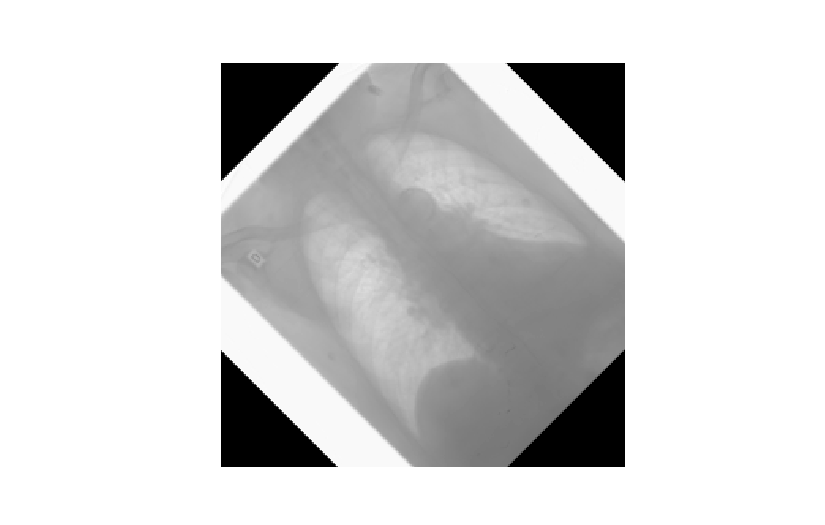
\includegraphics{Examen0003_files/figure-pdf/fig-Image01-2.pdf}

}

\caption{\label{fig-Image01}}

\end{figure}%

\begin{enumerate}
\tightlist
\item
  (10 Puntos) ¿Cuales de las siguientes operaciones no se puede realizar
  con la función warpAffine

  \begin{enumerate}
  \tightlist
  \item
    Escalamiento
  \item
    Traslación.
  \item
    Convolución.
  \item
    Transformación Gamma.
  \end{enumerate}
\end{enumerate}

\end{document}
